\section{Basic protocol 1: Explore the content of the ELM
DB}\label{basic-protocol-1-explore-the-content-of-the-elm-db}

The core of the ELM database is a repository of manually annotated
motifs and instances. As of December 2016, ELM contains over 260 motif
classes categorized into 6 different types: DOC (docking), LIG (Ligand
binding), DEG (degradation), CLV (cleavage), MOD (post translational
modifications), and TRG (targeting/anchoring) motifs (Figure
functional\_classification\_of\_SLiMs). These motifs are derived from
various types of experiments reported in literature. Each manually
annotated motif also has a set of bona fide instances (occurrences) of
this motif. Currently, there are over 3000 annotated instances annotated
from over 2500 publications. The motif classes and motif instances have
been uploaded by a large group of annotators from around the globe. The
complete catalogue of manually curated data can be searched, browsed and
explored on the ELM website

\subsection{Database content overview}\label{database-content-overview}

\begin{figure}[h!]
\centering
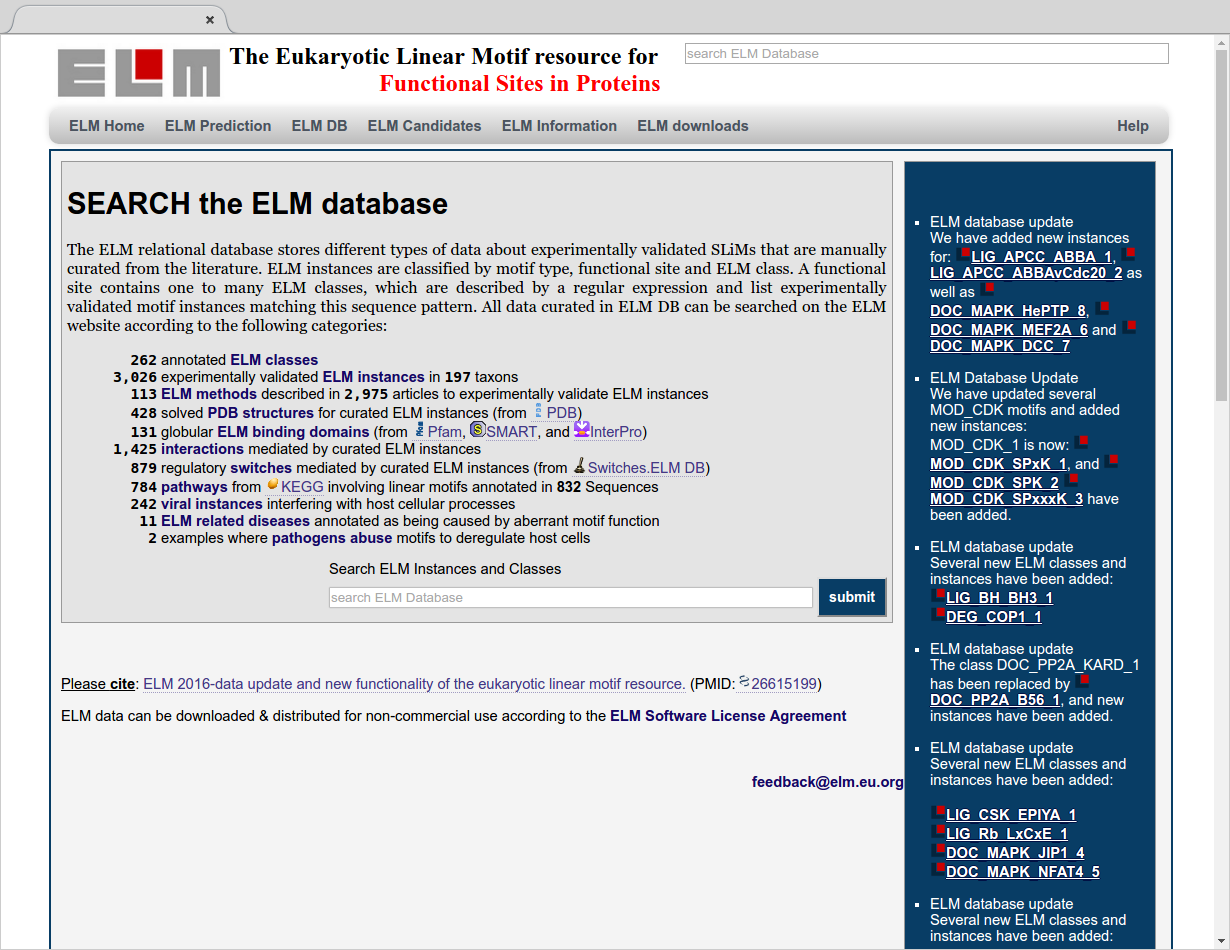
\includegraphics[width=\textwidth]{Figures/TP53_2/stats.png} 
\caption{
\textbf{Figure TP53-BP2-1}
The ELM database overview page (http://elm.eu.org/search.db).
}
\end{figure}

Step 1. Go to http://elm.eu.org and click on the tab ``ELM DB'' to
explore the content of the different types of data about experimentally
validated ELMs that were manually curated from the literature (Figure
TP53-BP2-1). This page contains a brief summary of the database content,
as well as the number of links to third-party databases. The table gives
an overview of the type and amount of information stored in the
database. Each line contains at least one link which will take you to
the corresponding contents page (eg. ``ELM instances'').

\begin{figure}[h!]
\centering
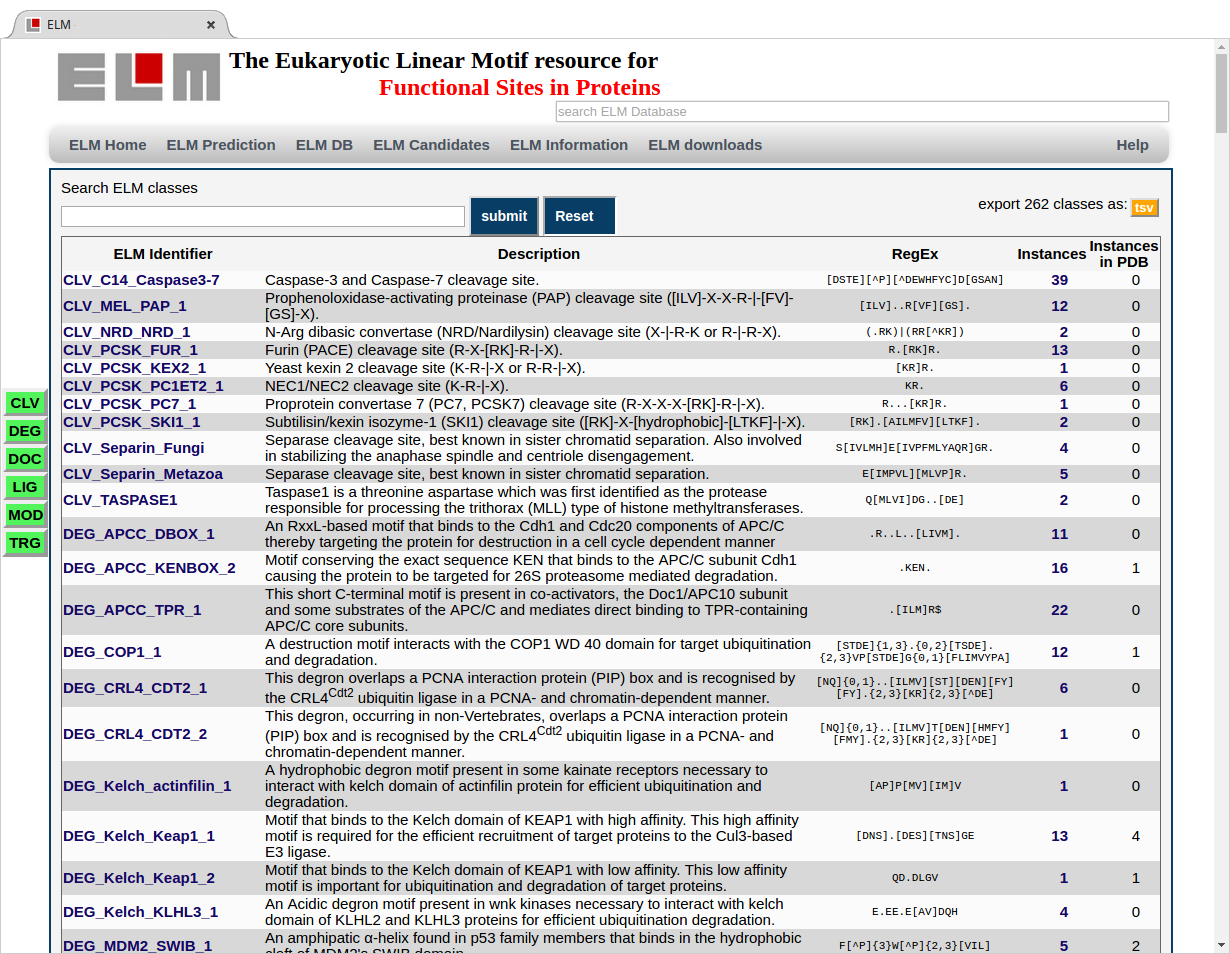
\includegraphics[width=\textwidth]{Figures/TP53_2/elms.png} 
\caption{
\textbf{Figure TP53-BP2-2}
The list of all motifs in the ELM database.
}
\end{figure}

Step 2. Click on the sub-menu ``ELM classes'' in ``ELM DB'' to see the
page with all of the ELM classes (Figure TP53-BP2-2). For each class,
the following information is provided: ELM identifier, short
description, regular expression, number of instances annotated for each
class, and number of structures available. For details on each class,
click on the ELM identifier; to get a list of annotated instances for an
individual class, click on the number of instances.

\sdesc{
Use the search bar at the top of the page to filter for certain motif
classes. For example, typing ``MAPK'' and hitting submit will perform a
full-text search on all motif classes in the ELM database containing the
term ``MAPK''. The green buttons on the left can also be used to filter
this table. For example, toggling the ``DOC'' button will remove all
``DOC'' classes from the table (and clicking it again will bring them
back). Lastly, the yellow tsv link can be used to export all motif
classes as a ``tab separated values'' file.
}

\begin{figure}[h!]
\centering
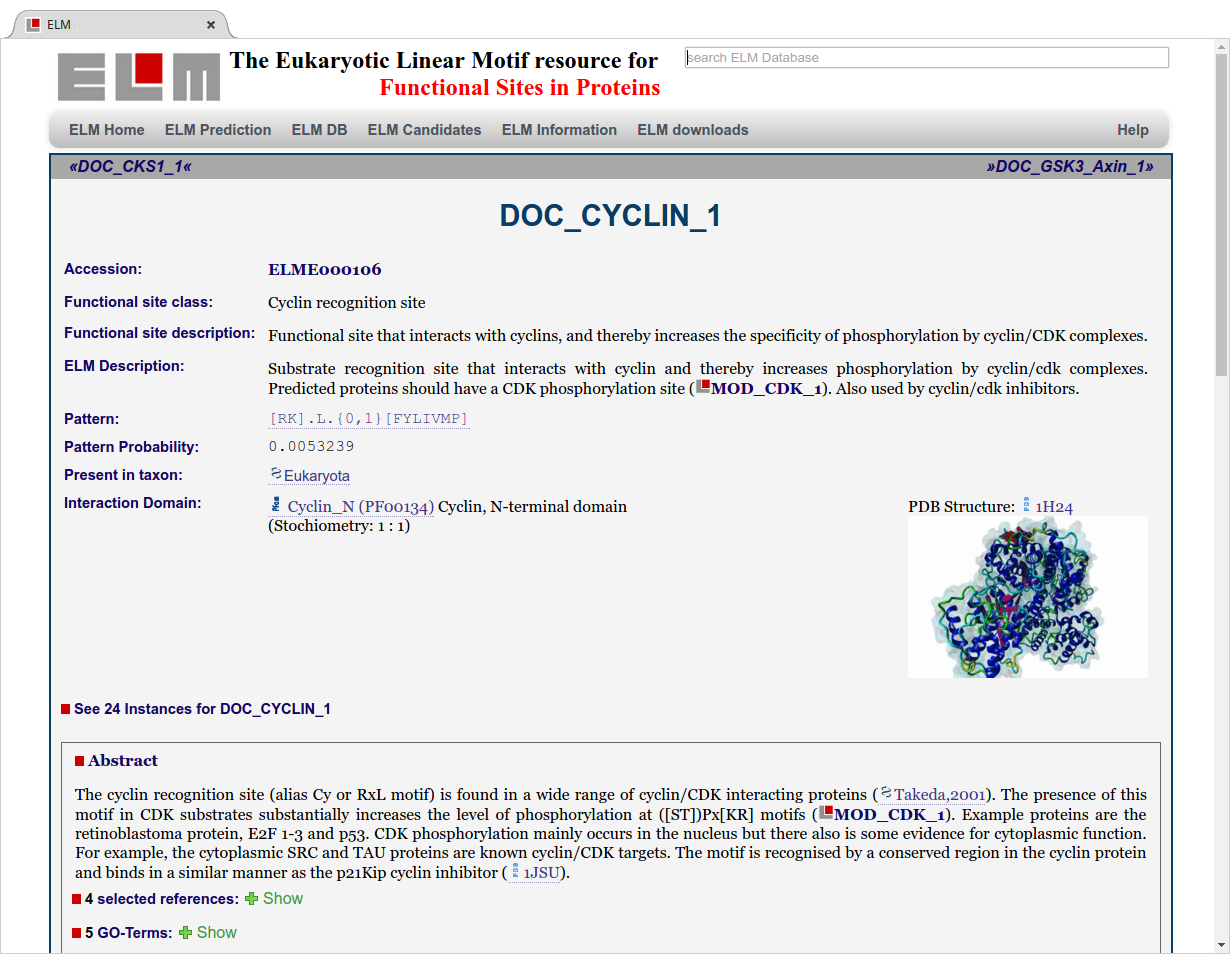
\includegraphics[width=\textwidth]{Figures/TP53_1/doc_cyclin_1_class.png}
\caption{
\textbf{Figure TP53-BP1- 4} 
The motif details page for
``DOC\_CYCLIN\_1''. This page contains all of the manual annotation
details for the DOC\_CYCLIN\_1 motif, the biological background
summarized from the scientific literature including links to the primary
literature and to external resources (Pubmed (\cite{27899561}),
GeneOntology (\cite{27899567}), PDB (\cite{12037327}) and more).
}
\end{figure}

Step 3. Search the table for the term ``DOC\_CYCLIN\_1'' and click on
its link to navigate to the page with details about the
``DOC\_CYCLIN\_1'' motif class (Fig TP53-BP1-4). This page contains a
description of the functional site class (a Cyclin recognition site),
and a short description of the ELM and its regular expression, as well
as a probability score, the taxonomic distribution of the motif and
which domain (if any) is responsible for the interaction.

\sdesc{
The probability score is the probability that the regular expression
represents a random selection of amino acids (similar to an information
content score). A lower score indicates that the motif pattern is more
difficult to find by chance in a random sequence.
}

Step 4. Scroll further down the ``DOC\_CYCLIN\_1'' page (Fig TP53-BP1-5)
to view more details about the manually annotated data and instances in
the database (to the text box starting with the ``Abstract''). The
``abstract'' contains a more detailed description of the motif
annotation. Click on the ``Show'' button next to the ``selected
references'' header for a list of publications relevant to this motif.
Click on ``Show'' next to ``GO terms'' for a complete list of all GO
terms annotated for this motif.

Step 5. Scroll further down the ``DOC\_CYCLIN\_1'' page (Fig TP53-BP1-5)
to view the ``Instances'' header. This table contains the list of all
annotated instances in the database of this motif. This includes the
protein identifier, the start and end positions of the instance, the
specific sequence matching the regular expression and the logic of the
instance. The ``\# Ev.'' indicates the number of experimental evidences
associated with the annotation (see section XXX below). Organism is the
species in which the protein is found. Lastly the ``Notes'' column
contains links to any ``interactions'' or ``switches'' present in the
database, as well as links to PDB if this structure exists in PDB.

\subsubsection{Browsing annotated
instances}\label{browsing-annotated-instances}

\begin{figure}[h!]
\centering
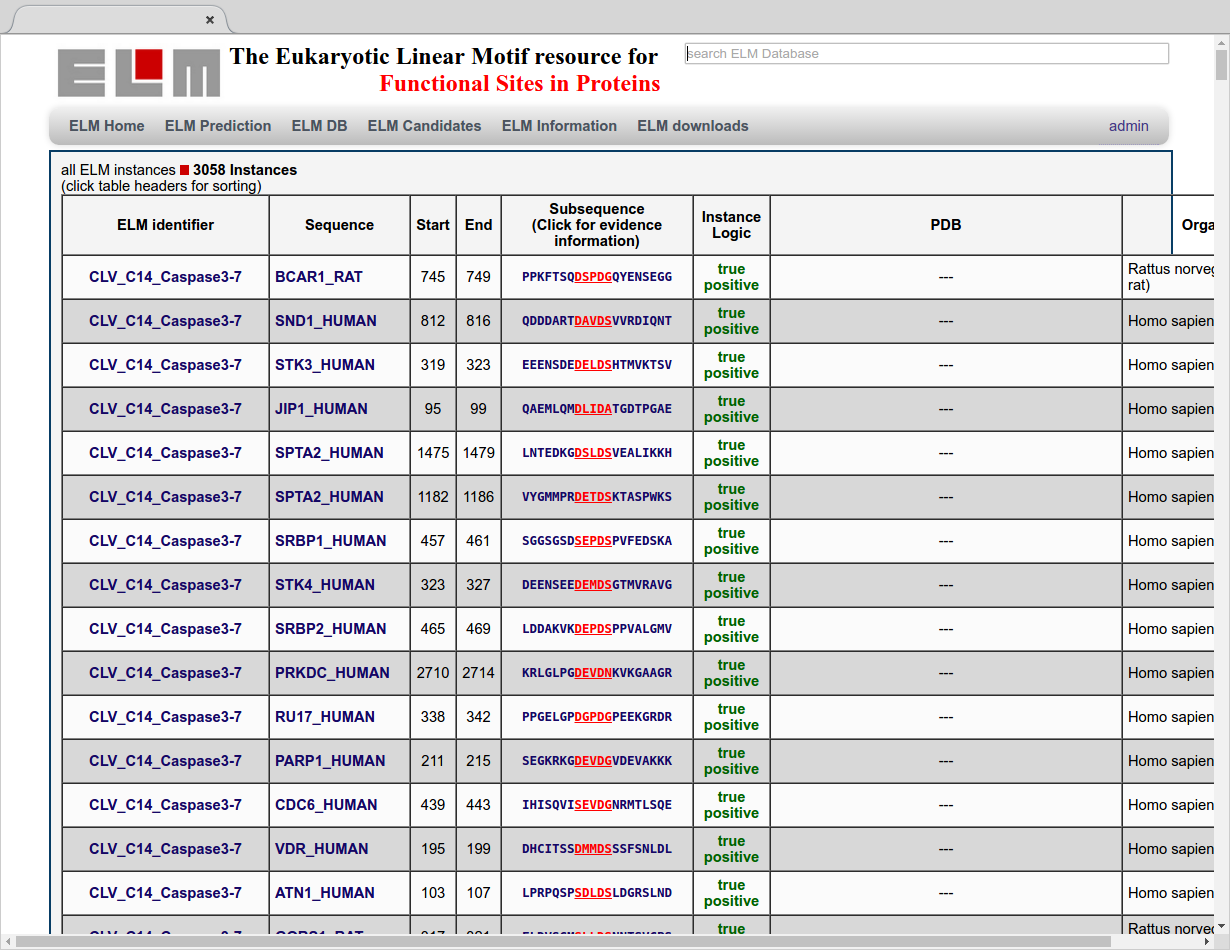
\includegraphics[width=\textwidth]{Figures/TP53_2/instances.png} 
\caption{
\textbf{Figure TP53-BP2-3}
The list of all instances in the ELM database.
}
\end{figure}

Step 6. Click on the sub-menu ``ELM instances'' in ``ELM DB'' to go to
the page which lists all of the instances in the database (Figure
TP53-BP2-3). This table contains a list of all instances in the
database.

\sdesc{
Use the search filters at the top of the page to limit the results by a
full text search, by instance logic, or organisms. Similar to the ELM
classes page (previous step) these results can be filtered by motif
class using the green toggle filters on the left hand side. Lastly, the
yellow buttons at the top of the page can be used to download the
instances in the following formats: gff, pir, fasta or tsv.
}

\begin{figure}[h!]
\centering
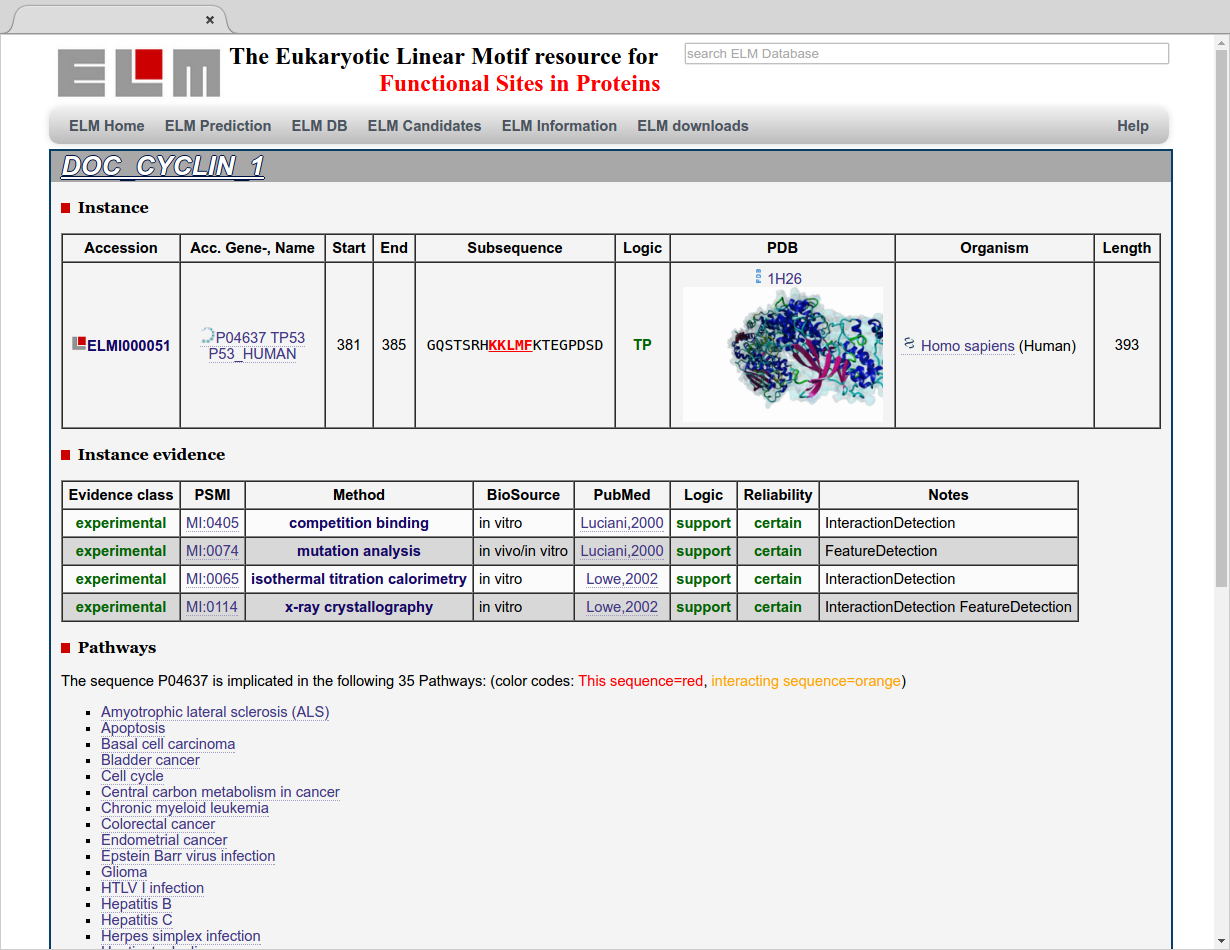
\includegraphics[width=\textwidth]{Figures/TP53_1/doc_cyclin_1_instance.png}
\caption{
\textbf{Figure TP53-BP1- 5}
The instance details page for the
``DOC\_CYCLIN\_1'' instance annotated for protein P53\_HUMAN with
start/end position ``381-385''. This page also contains links to many
external databases including Uniprot (\cite{25348405}), PDB
(\cite{12037327}), NCBI taxonomy, Pubmed (\cite{27899561}), and KEGG
Pathways (\cite{26476454}), as well as the PSI-MI controlled vocabulary
(\cite{17925023}).
}
\end{figure}

Step 7. Type ``p53\_human'' in the search box to search for ELM
Instances in this protein. Find the row for the ELM class
``DOC\_CYCLIN\_1'' and click on the startposition ``381'' to go to the
instance details page of this instance. The top part of the page
contains details about the instance and the protein it was identified
in.

Step 8. Scroll down to the ``Instance Evidence'' header to view details
on the experimental evidence used to annotate this instance. This table
also contains the ``evidence class'', and descriptions of the methods
used from PSI-MI (\cite{17925023}) as well as the Literature references
in which the experiments were published.

\sdesc{
(Here we should explain what ``evidence class'', ``biosource'',
``Logic'', ``Reliability'' and ``Notes'' actually mean).
}

\subsection{Details on molecular switches, motif-mediated pathways and
other external
resources.}\label{details-on-molecular-switches-motif-mediated-pathways-and-other-external-resources.}

Step 9. Scroll further down to the header ``Pathways'' to view pathway
information. This is a list of all of the pathways in which the protein
p53 is known to be involved (according to KEGG). Click on a pathway to
see the localization of p53 in the corresponding KEGG pathway.

\begin{figure}[h!]
\centering
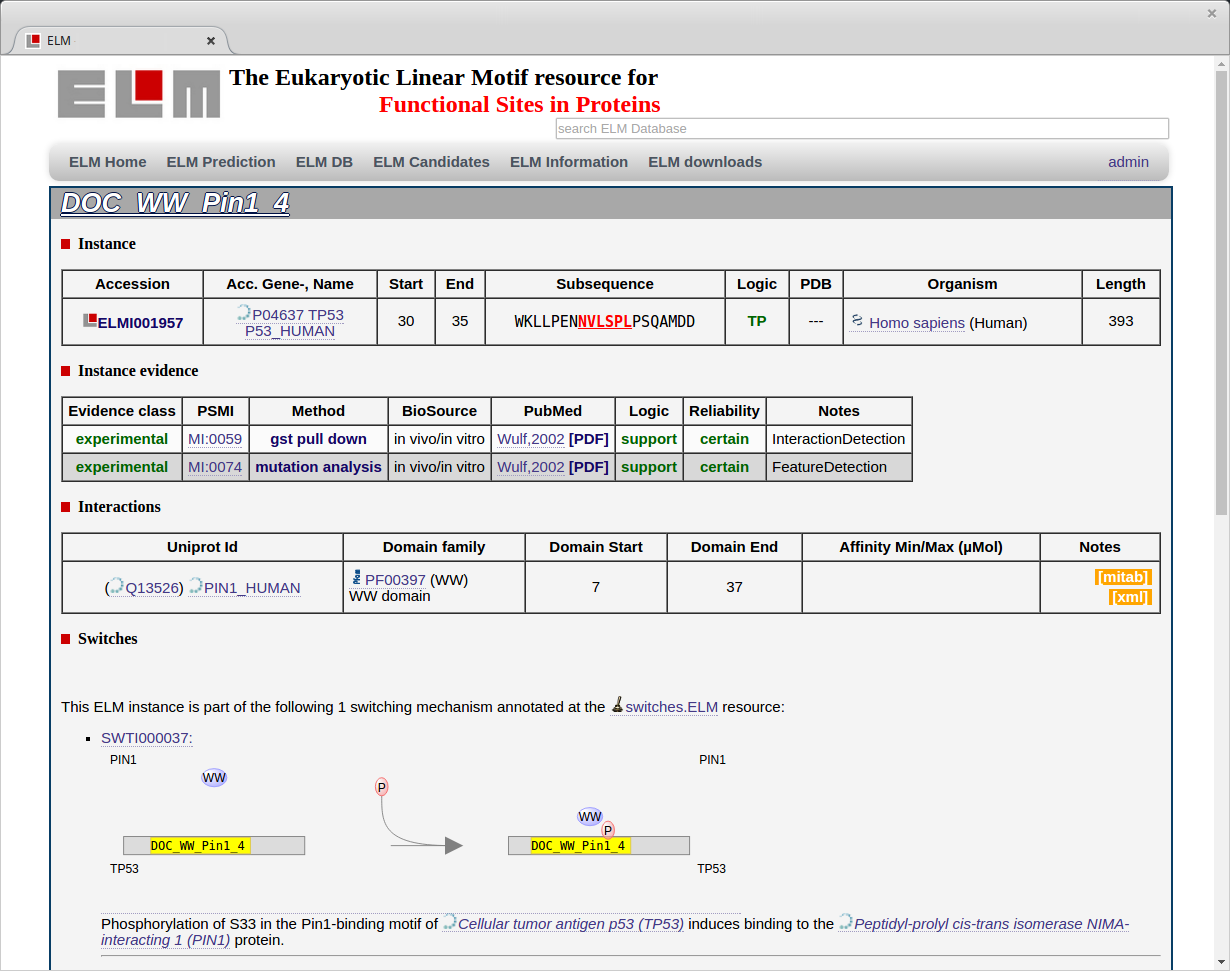
\includegraphics[width=\textwidth]{Figures/TP53_1/doc_ww_pin_1_4_instance.png}
\caption{
\textbf{Figure TP53-BP1-6} The instance details page for the
``DOC\_WW\_Pin1\_4'' instance found in P53 with start/end position
``30-35''.
}
\end{figure}

Step 10. Repeat the previous search by clicking on the sub-menu ``ELM
instances'' in ``ELM DB'' and type ``p53\_human'' in the search box.
This time, try to find the ELM instance ``DOC\_WW\_Pin1\_4'' motif with
the start/end position ``30-35'' (You can sort the table by clicking on
the header lines eg. on ``Start'' to sort by startposition ). Click on
the start/endposition or the subsequence which will take you to the
details page as shown in Fig TP53-BP1-6. This page is similar to that
described for the P53 instance ``DOC\_CYCLIN\_1'' (Fig TP53-BP1-5);
additionally, for this instance there is information available about its
interaction partner and a molecular switch which is mediated by this
motif instance.

Step 11. Scroll down to the ``Interactions'' header to view information
about this instance's interactions (Fig TP53-BP1-6). This instance
interacts with PIN1\_Human via the ``WW'' domain (PFAM identifier
PF00397; found on position 7--37 in PIN1\_Human). If available, binding
affinities are also shown here. Interaction data is made available in
Mitab and xml format (\cite{17925023}).

Step 12. Scroll further down to the ``Switches'' section for a brief
overview of the switches details of this instance obtained form
``switches.ELM'' (\cite{23550212}) (Fig TP53-BP1-6). This particular
instance is involved in the switch phosphorylating P53. Clicking on the
diagram will open an external link to the ``switches.ELM'' website.

\begin{figure}[h!]
\centering
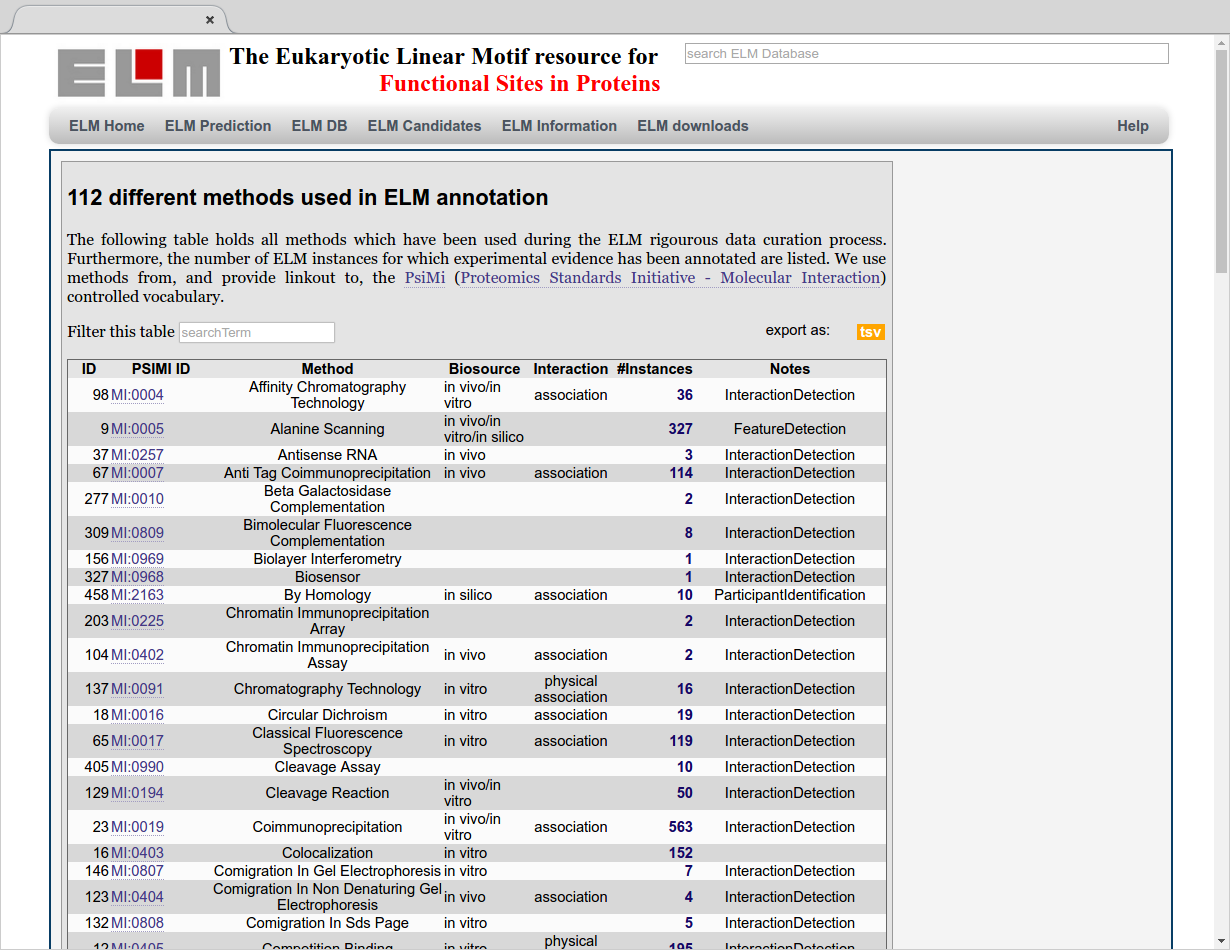
\includegraphics[width=\textwidth]{Figures/TP53_2/methods.png} 
\caption{
\textbf{Figure TP53-BP2-4}
The list of all experimental methods used in the ELM
database.
}
\end{figure}

Step 13. Click on the sub-menu ``ELM methods'' in ``ELM DB'' to see a
list of all experimental methods which have been used to identify motifs
and instances (figure TP32-BP2-4). This table shows the internal method
identifier in the first column, a link to the corresponding entry in the
PSI-MI database (\cite{17925023}), and the method name as annotated by
the PSI-MI controlled vocabulary, as well as the type of experiment (in
vitro/in vivo). Clicking on the link in the ``instances'' column will
list all instances annotated using that method.

\sdesc{
The filter bar on the top page can be used to filter the list of
methods. The \emph{tsv} link creates a downloadable file in ``tab
separated values'' format.
}

\begin{figure}[h!]
\centering
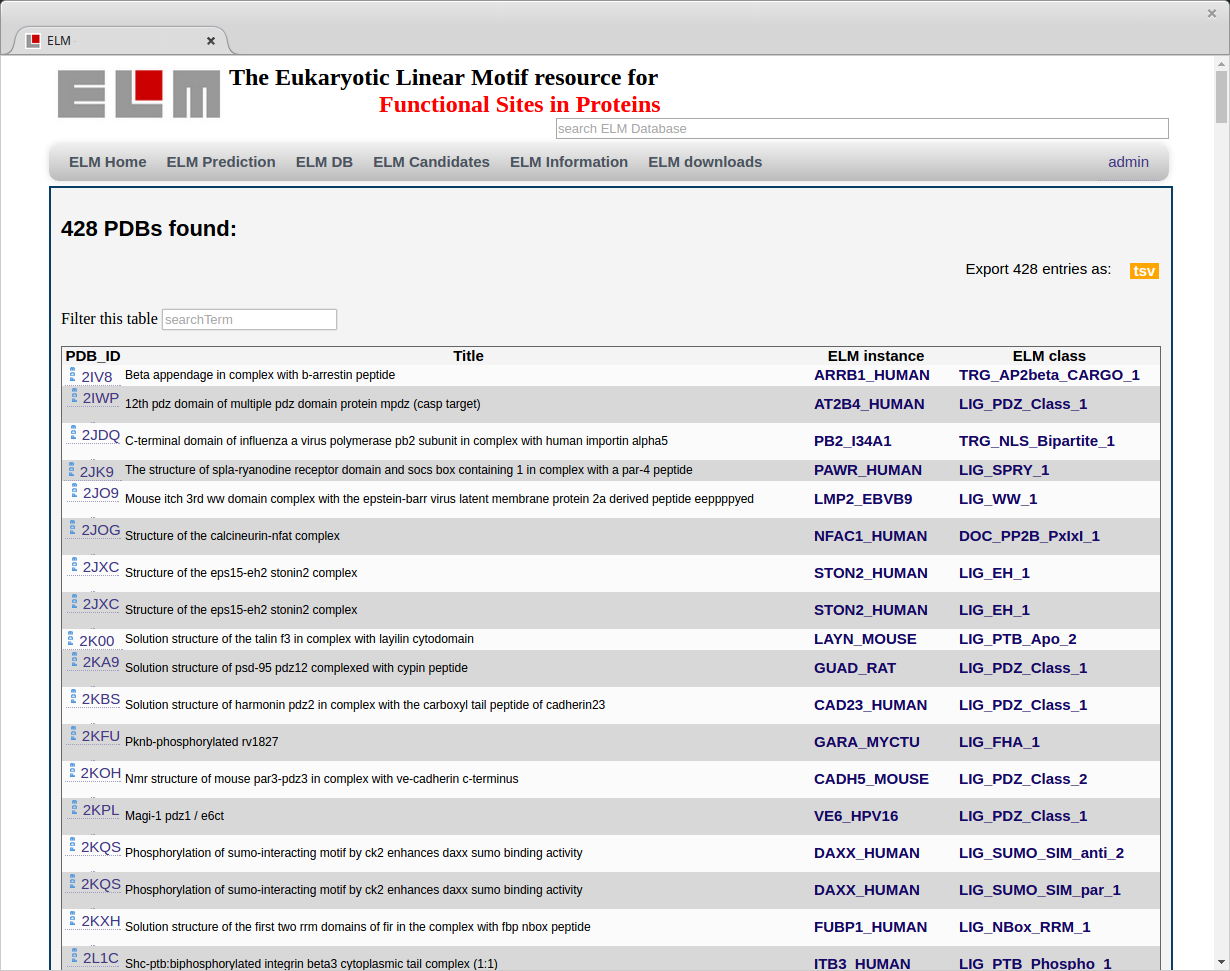
\includegraphics[width=\textwidth]{Figures/TP53_2/pdbs.png} 
\caption{
\textbf{Figure TP53-BP2-5}
The list of all known structures in PDB also in ELM.
}
\end{figure}

Step 14. Click on the sub-menu ``ELM pdb structures'' in ``ELM DB'' to
see a list of all macromolecular structures in the ELM database (Figure
TP53-BP2-5). Structures annotated in ELM ideally (but not always) show
both interaction partners, motif and domain. This page also contains
links to RCSB (\cite{12037327}), the individual instance and the motif
class of that instance.

\sdesc{
The filter bar on the top page can be used to filter the list of
structures shown . The \emph{tsv} link creates a downloadable file in
``tab separated values'' format. The \emph{tsv} file contains the PDB
id, uniprot name, and ELM class.
}

\begin{figure}[h!]
\centering
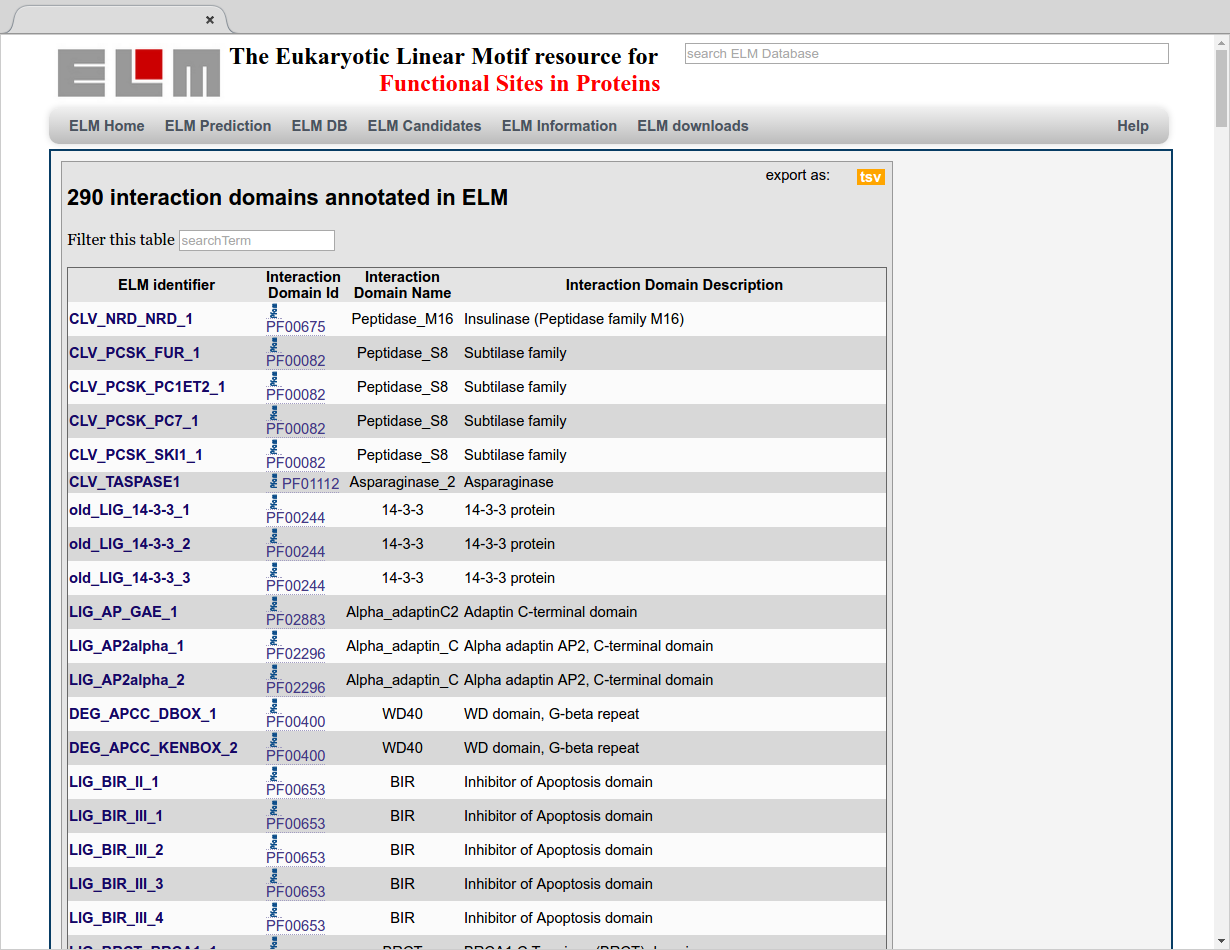
\includegraphics[width=\textwidth]{Figures/TP53_2/interactiondomains.png}
\caption{
\textbf{Figure TP53-BP2-6} A list of all interactions annotated in the
database.
}
\end{figure}

Step 15. Click on the sub-menu ``ELM binding domains'' in ``ELM DB'' to
see a complete list of all the interaction domains in ELM (Figure
TP53-BP2-6). This table shows the ELM classes which have been annotated
with a corresponding interaction domain. This table shows the ELM class,
a link to the Pfam (\cite{26673716}) / SMART (\cite{25300481}) /
InterPro (\cite{27899635}) domain, as well as the name of the
interacting domain followed by a brief description.

\sdesc{
The filter bar on the top page can be used to filter the list of
interactions shown. The \emph{tsv} link creates a downloadable file in
``tab separated values'' format.
}

\subsection{Links to external
resources}\label{links-to-external-resources}

\begin{figure}[h!]
\centering
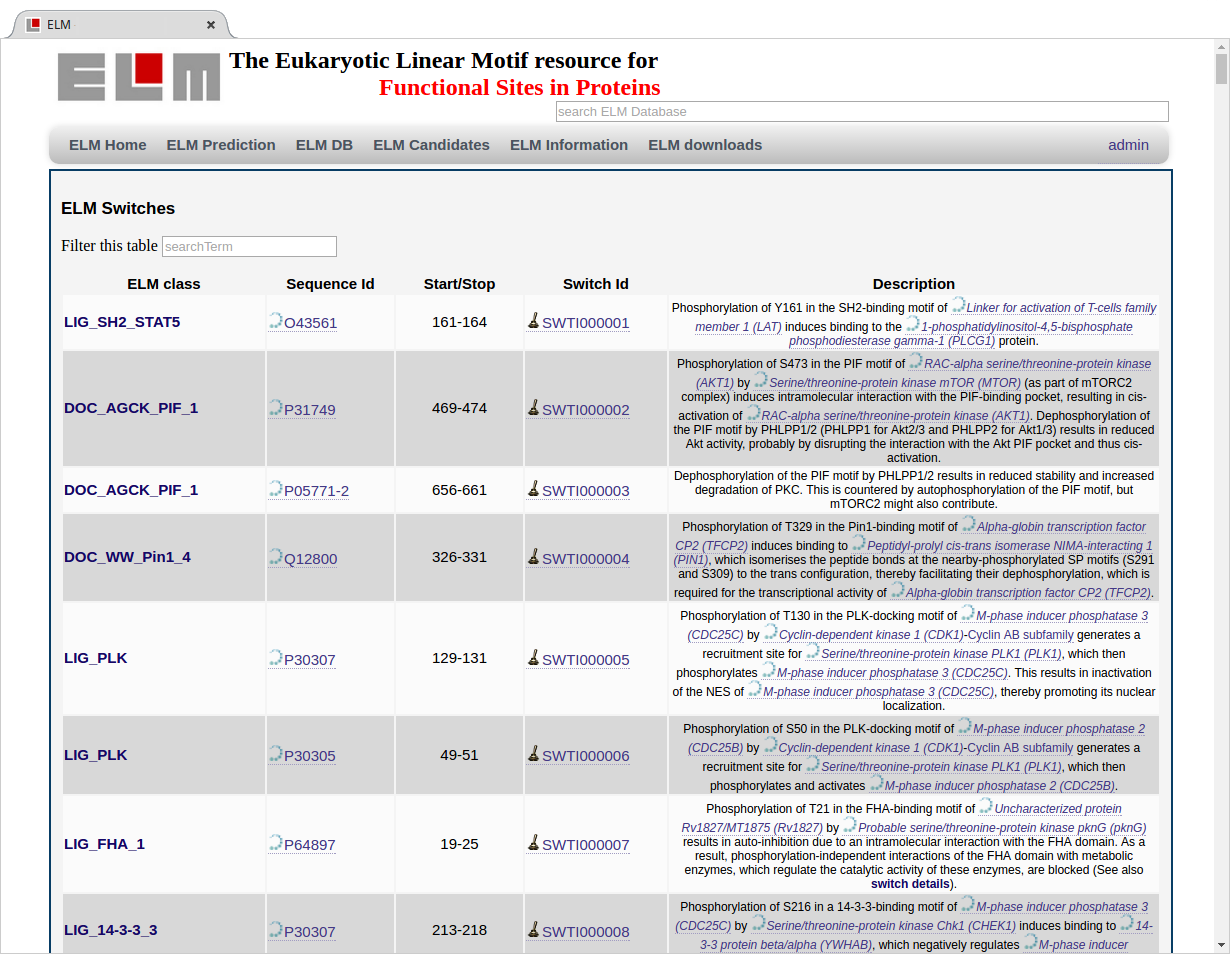
\includegraphics[width=\textwidth]{Figures/TP53_2/switches.png} 
\caption{
\textbf{Figure TP53-BP2-7}
A list of all switches annotated in ELM.
}
\end{figure}

Step 16. Click on the sub-menu ``ELM switches'' in ``ELM DB'' to see a
complete list of all the switches in ELM (Figure TP53-BP2-7). This table
shows the motif class, contains a link to Uniprot, and the start and
stop positions of the motif mediating the switch. The last two columns
have links to switches.ELM, and a brief description of the switch also
taken from switches.ELM (\cite{23550212}).

\sdesc{
The filter bar on the top page can be used to quickly filter the list of
interactions shown.
}

\subsection{Exploring KEGG pathways from
ELM}\label{exploring-kegg-pathways-from-elm}

\begin{figure}[h!]
\centering
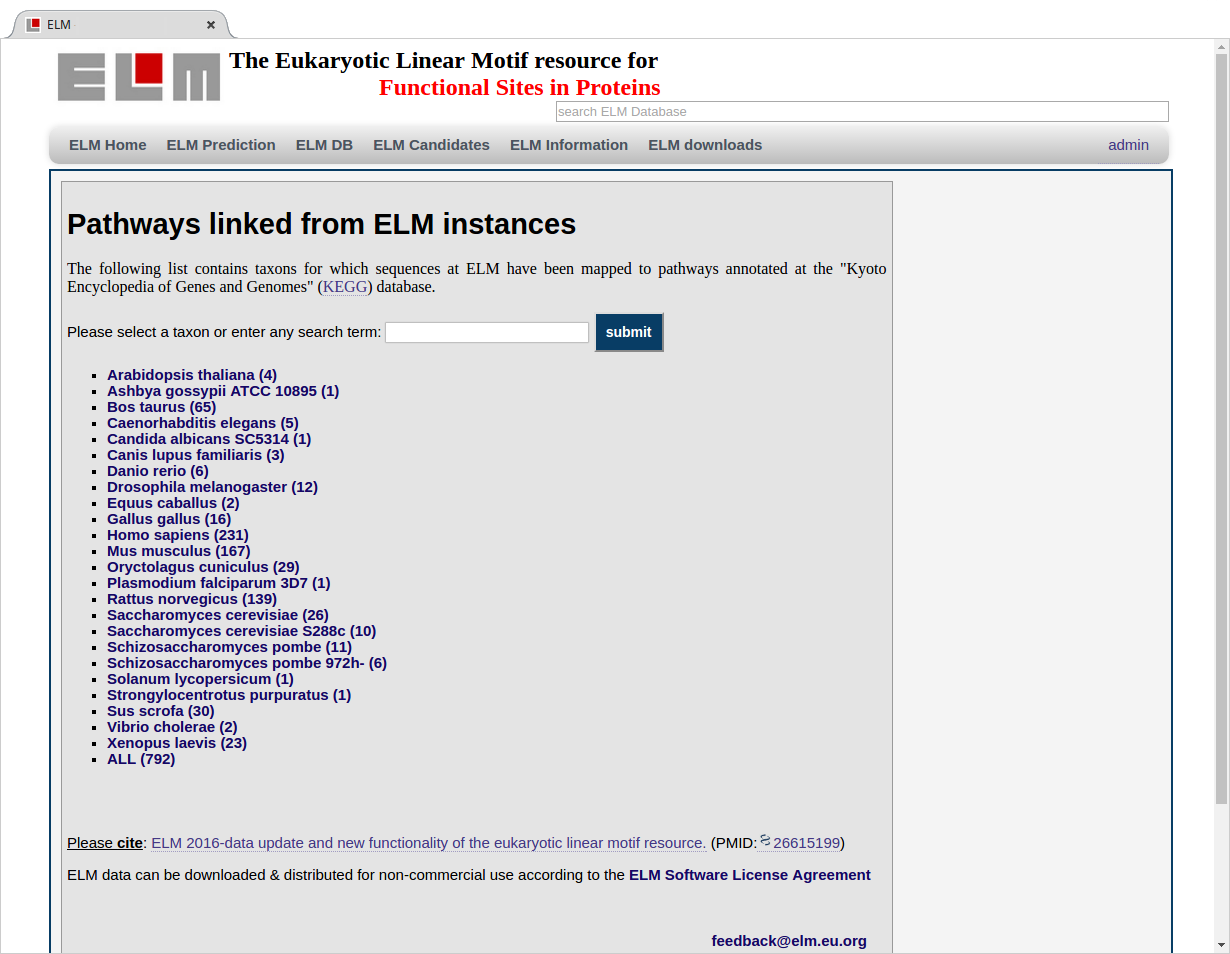
\includegraphics[width=\textwidth]{Figures/TP53_2/pathways.png} 
\caption{
\textbf{Figure TP53-BP2-9}
A list of all Pathways from KEGG with proteins in ELM.
}
\end{figure}

Step 17. Click on the sub-menu ``ELM pathways'' in ``ELM DB'' to see a
list of all pathways contained in ELM (Fig. TP53-BP2-9). Pathways are
from the ``Kyoto Encyclopedia of Genes and Genomes'' (KEGG
\cite{26476454}) database mapped to ELM instances. Click on a species
(for example ``Homo sapiens'') for a complete list of all Human pathways
which have a protein annotated in ELM, and links to the pathways on
KEGG.

\begin{figure}[h!]
\centering
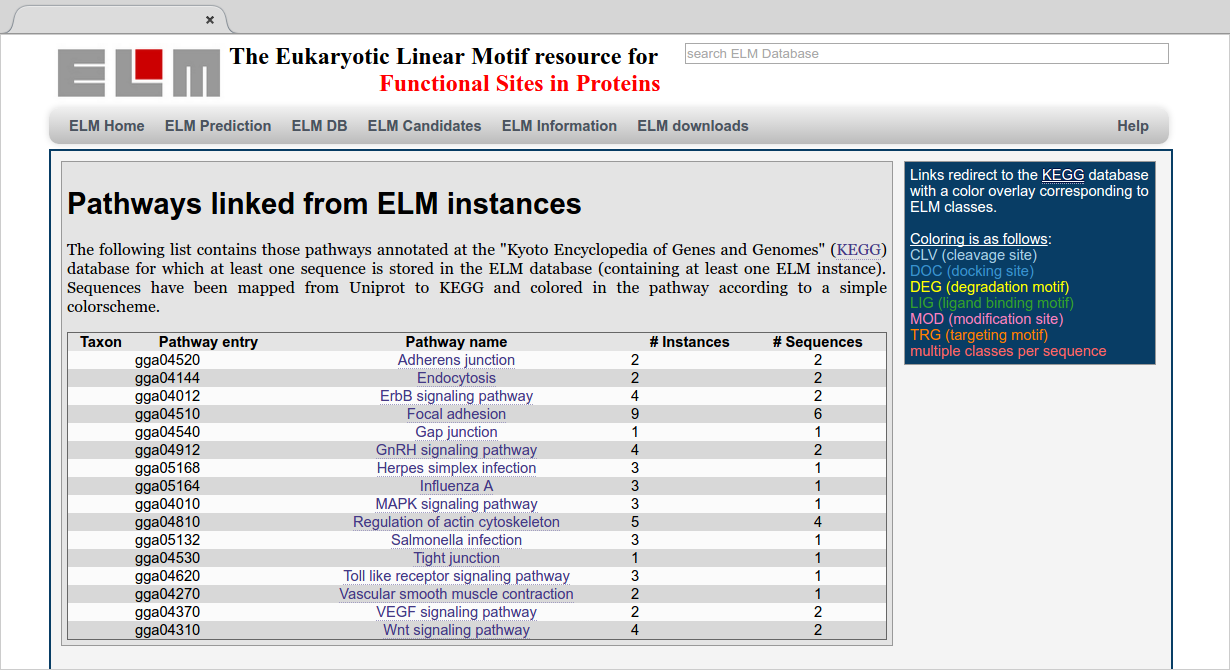
\includegraphics[width=\textwidth]{Figures/TP53_2/pathways_example.png} 
\caption{
\textbf{Figure TP53-BP2-10}
A list of all pathways in Gallus Gallus
}
\end{figure}

Step 18. On the ``ELM pathways'' page (Fig. TP53-BP2-9) click on the
link ``gallus gallus'' to navigate to the page containing all pathways
annotated for chicken. This page contains links to all KEGG pathways for
the taxon \emph{gallus gallus} with annotated instances in the ELM
database.

\begin{figure}[h!]
\centering
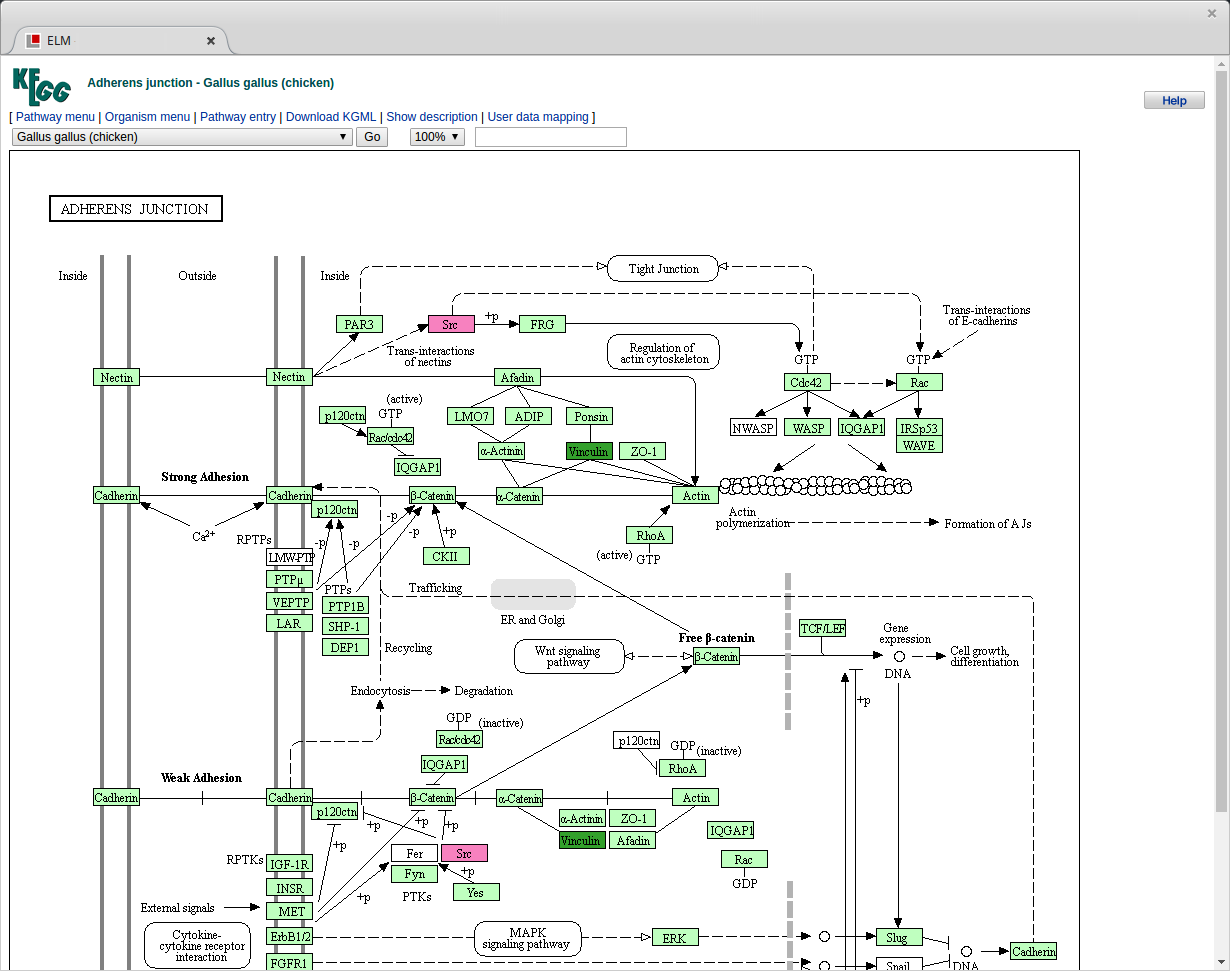
\includegraphics[width=\textwidth]{Figures/TP53_2/pathways_kegg.png} 
\caption{
\textbf{Figure TP53-BP2-11}
A list of all annotated pathways for taxon \emph{gallus gallus}
}
\end{figure}

Step 19. One the page with chicken pathways (Fig. TP53-BP2-10) click on
``Adherens junction'' to the KEGG entry for this pathway, with proteins
color overlay corresponding to ELM classes (see the color legend right
side of figure TP53-BP2-10).

\subsection{Infections and Diseases}\label{infections-and-diseases}

\begin{figure}[h!]
\centering
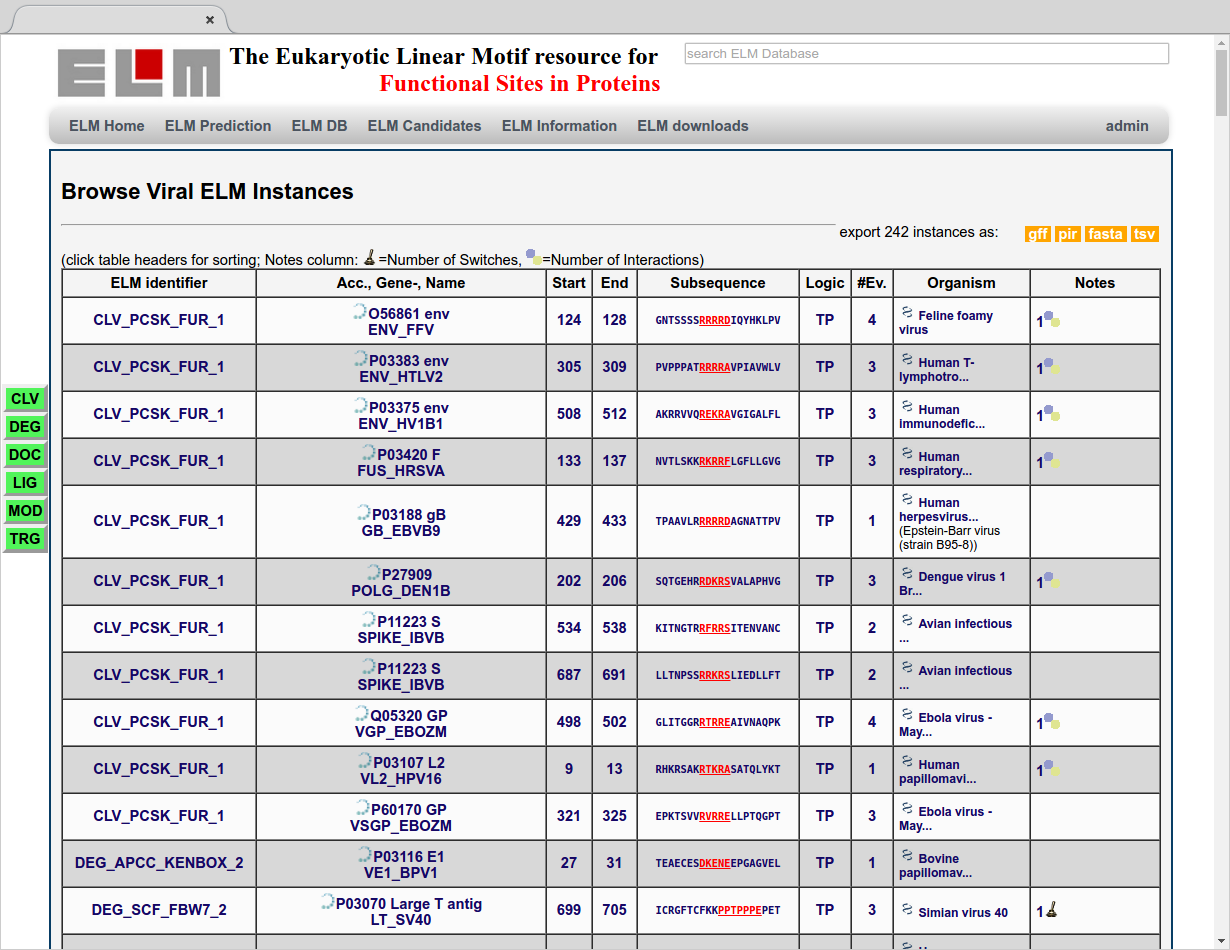
\includegraphics[width=\textwidth]{Figures/TP53_2/viruses.png} 
\caption{
\textbf{Figure TP53-BP2-11}
A Table of the ELM instance abused by viruses
}
\end{figure}

Step 20. Click on the sub-menu ``ELM virus instances'' in ``ELM DB'' to
see a list of all instances in ELM that have been annotated as being
abused by viruses (Fig TP53-BP2-9). The columns are identical to those
listed in section XXX step YYY (Figure ZZZZ).

\sdesc{
The green buttons on the left can be used to filter this table by motif
class. Click on the yellow links on the top right of the page to
download the (complete) table in gff, pir, fasta or tsv format. (See
section XXX for a description of these formats.)
}

\begin{figure}[h!]
\centering
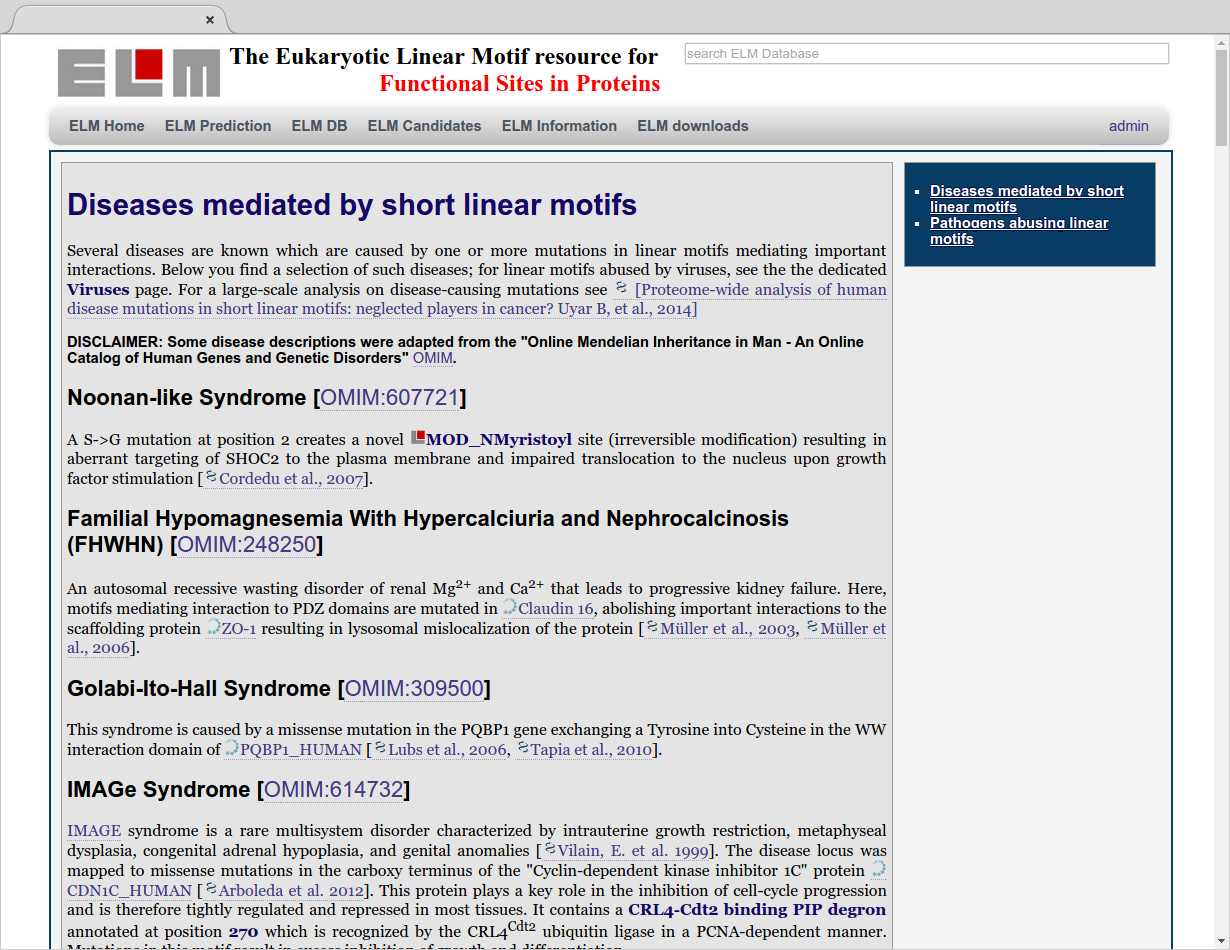
\includegraphics[width=\textwidth]{Figures/TP53_2/diseases.png}
\caption{
\textbf{Figure TP53-BP2-8}
A list of all diseases in ELM.
}
\end{figure}

Step 21. Click on the sub-menu ``ELM diseases'' in ``ELM DB'' to see a
list of all motif classes that have been annotated with a disease.
Disease information is taken from the OMIM database.

\sdesc{
This table also includes the diseases found under the ``ELM pathogenic
abuse'' menu in ``ELM DB''. (right?)
}

